% Author: Izaak Neutelings (Februari, 2020)
% http://texample.net/tikz/examples/tag/circuitikz/
% http://texample.net/tikz/examples/circuitikz/
% https://www.overleaf.com/learn/latex/CircuiTikz_package
% http://texdoc.net/texmf-dist/doc/latex/circuitikz/circuitikzmanual.pdf
% http://repositorios.cpai.unb.br/ctan/graphics/pgf/contrib/circuitikz/circuitikzmanual.pdf
\documentclass[border=3pt,tikz]{standalone}
\usepackage{amsmath} % for \dfrac
\usepackage{physics}
\usepackage{tikz,pgfplots}
\usepackage[siunitx]{circuitikz} %[symbols]
\usepackage[outline]{contour} % glow around text
\usetikzlibrary{arrows,arrows.meta}
\usetikzlibrary{decorations.markings}
\tikzset{>=latex} % for LaTeX arrow head
\usepackage{xcolor}
\colorlet{Icol}{blue!50!black}
\colorlet{Ccol}{orange!90!black}
\colorlet{Rcol}{green!50!black}
\colorlet{Lcol}{blue!50!black}
\colorlet{loopcol}{red!90!black!25}
\colorlet{pluscol}{red!60!black}
\colorlet{minuscol}{blue!60!black}
% \newcommand\EMF{\mathcal{E}} %\varepsilon}
% \contourlength{1.5pt}
% \tikzstyle{EMF}=[battery1,l=$\EMF$,invert]
% \tikzstyle{internal R}=[R,color=Rcol,Rcol,l=$r$,/tikz/circuitikz/bipoles/length=30pt]
% \tikzstyle{loop}=[->,red!90!black!25]
% \tikzstyle{loop label}=[loopcol,fill=white,scale=0.8,inner sep=1]
% \tikzstyle{thick R}=[R, color=Rcol,thick,Rcol,l=$R$]
% \tikzstyle{thick C}=[C,thick,color=Ccol,Ccol,l=$C$]
% \tikzstyle{thick L}=[L,thick,color=Lcol,Lcol,l=$L$,/tikz/circuitikz/bipoles/length=56pt]
% \tikzstyle{myswitch}=[closing switch,line width=0.3] %-{Latex[length=3]},

\ctikzset{bipoles/generic/width=1.2, bipoles/generic/height=0.5}

% \newcommand{\myvoltmeter}[2] 
% {  % #1 = name , #2 = rotation angle
%   \begin{scope}[transform shape,rotate=#2]
%   \draw[thick] (#1)node(){$\mathbf V$} circle (11pt);
%   \draw[rotate=45,-latex] (#1)  +(-17pt,0) --+(17pt,0);
%   \end{scope}
% }

\begin{document}


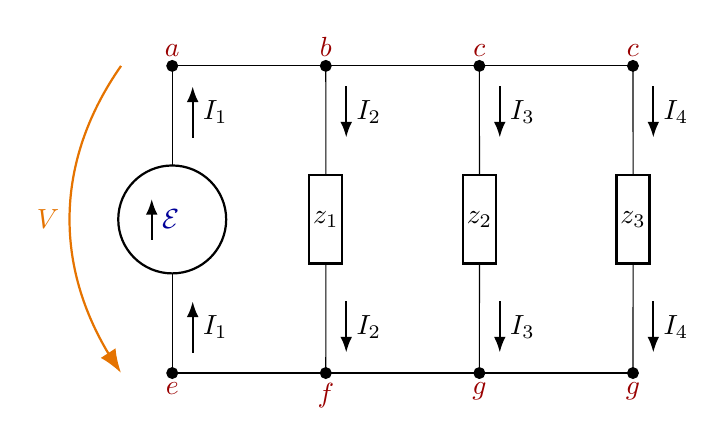
\begin{tikzpicture}[scale=1.3]


    \coordinate (P1) at (0, 0);
    \coordinate (P2) at (1.5, 0);
    \coordinate (P3) at (3, 0);
    \coordinate (P4) at (4.5, 0);
    \coordinate (P5) at (0, -3);
    \coordinate (P6) at (1.5, -3);
    \coordinate (P7) at (3, -3);
    \coordinate (P8) at (4.5, -3);
    
    \filldraw [black] (P1) circle (1.5pt);
    \filldraw [black] (P2) circle (1.5pt);
    \filldraw [black] (P3) circle (1.5pt);
    \filldraw [black] (P4) circle (1.5pt);
    \filldraw [black] (P5) circle (1.5pt);
    \filldraw [black] (P6) circle (1.5pt);
    \filldraw [black] (P7) circle (1.5pt);
    \filldraw [black] (P8) circle (1.5pt);

    \draw (P1) -- (P4);
    \draw (P5) -- (P8);

    \draw (P5) node [below, pluscol] {$e$} -- (P1) node [above, pluscol] {$a$};
    \filldraw[fill=white, thick] (0, -1.5) circle (15pt);
    \draw[-{Latex[length=2mm]},  thick] (-0.2, -1.7) to node [midway, right, minuscol] {$\mathcal{E}$} (-0.2, -1.3); 
    \draw[-{Latex[length=2mm]},  thick] (0.2, -0.7) -- (0.2, -0.2) node [midway, right] {$I_1$};
    \draw[-{Latex[length=2mm]},  thick] (0.2, -2.8) -- (0.2, -2.3) node [midway, right] {$I_1$};


    \draw[-{Latex[length=3mm]}, Ccol,  thick, bend left=-35] (-0.5, 0) to node [midway, left] {$V$} (-0.5, -3) ;

    \draw (P6) node[below, pluscol] {$f$} to[generic, name=z1] (P2) node [above, pluscol] {$b$};
    \node at (z1.center) {$z_1$}; 

    \draw[-{Latex[length=2mm]},  thick] (1.7, -0.2) -- (1.7, -0.7) node [midway, right] {$I_2$};
    \draw[-{Latex[length=2mm]},  thick] (1.7, -2.3) -- (1.7, -2.8) node [midway, right] {$I_2$};

    \draw (P7) node[below, pluscol] {$g$} to[generic, name=z2] (P3) node [above, pluscol] {$c$};
    \node at (z2.center) {$z_2$}; 

    \draw[-{Latex[length=2mm]},  thick] (3.2, -0.2) -- (3.2, -0.7) node [midway, right] {$I_3$};
    \draw[-{Latex[length=2mm]},  thick] (3.2, -2.3) -- (3.2, -2.8) node [midway, right] {$I_3$};

    \draw (P8) node[below, pluscol] {$g$} to[generic, name=z3] (P4) node [above, pluscol] {$c$};
    \node at (z3.center) {$z_3$}; 

    \draw[-{Latex[length=2mm]},  thick] (4.7, -0.2) -- (4.7, -0.7) node [midway, right] {$I_4$};
    \draw[-{Latex[length=2mm]},  thick] (4.7, -2.3) -- (4.7, -2.8) node [midway, right] {$I_4$};


    % \draw (P1) node[left, pluscol] {$a$} to[generic, name=g2] (P2) node [right, pluscol] {$b$};
    % \node at (g2.center) {$z_2$}; 

    % \draw[-{Latex[length=3mm]}, dashed, thick, bend left=-35] (P1) to node [midway, below] {$V_2$} (P2) ;

    % \draw (P2) to[generic, name=g3] (P3) node [right, pluscol] {$c$};
    % \node at (g3.center) {$z_3$}; 

    % \draw[-{Latex[length=3mm]}, dashed, thick, bend left=-35] (P2) to node [midway, left] {$V_3$} (P3) ;

    % \draw (P3) to[generic, name=g4] (P4) node [right, pluscol] {$d$};
    % \node at (g4.center) {$z_4$}; 

    % \draw[-{Latex[length=3mm]}, dashed, thick, bend left=-35] (P3) to node [midway, left] {$V_4$} (P4) ;

    % \draw (P4) to[generic, name=g5] (P5) node [left, pluscol] {$e$};
    % \node at (g5.center) {$z_5$}; 

    % \draw[-{Latex[length=3mm]}, dashed, thick, bend left=-35] (P4) to node [midway, above] {$V_5$} (P5) ;

    % \draw (P5) to[generic, name=g6] (P6) node [left, pluscol] {$f$};
    % \node at (g6.center) {$z_6$}; 

    % \draw[-{Latex[length=3mm]}, dashed, thick, bend left=-45] (P5) to node [midway, right] {$V_6$} (P6) ;

    % \draw (P6) -- (P7) node [left, pluscol] {$g$};
    % \filldraw[fill=white, thick] (0, -3.5) circle (15pt);
    % \draw[-{Latex[length=2mm]},  thick] (-0.2, -3.7) to node [midway, right, minuscol] {$\mathcal{E}$} (-0.2, -3.3); 

    % \draw[-{Latex[length=3mm]}, dashed, thick, bend left=-89] (P6) to node [midway, right] {$V_7$} (P7) ;

    % \draw (P7) to[generic, name=g1] (P1);
    % \node at (g1.center) {$z_1$}; 

    % \draw[-{Latex[length=3mm]}, dashed, thick, bend left=-45] (P7) to node [midway, right] {$V_1$} (P1) ;

    % \node [Icol, left] at (2, -4) {$\Gamma$};
    % \draw[-{Latex[length=2mm]}, Lcol, thick, bend left=45] (2, -4) to (2.5, -4.3) ;


    % \draw (-0.5, 0) to (-2, 0) to [thick L] (-2, 2) to[thick R] (2, 2) to [thick C] (2, 0) -- (0.5, 0); 

    % \draw[fill=white] (-0.5, 0) circle (2pt) node [yshift=-10] {$1$};
    % \draw[fill=white] (0.5, 0) circle (2pt) node [yshift=-10] {$2$};
    % \node [] (0, 0) {$V$};
    
\end{tikzpicture}

\end{document}